\documentclass{article}
\usepackage{ctex}
\usepackage{graphicx}
\begin{document}
	\title{对单词模糊查询问题的一些初步探索\\ 课题编号:161}
	\author{于宸锴\and 张子禾 \and 杨晨\and 指导教师:庄丽}
	\maketitle
	\section{引言}
	我们对单词模糊查询问题做了初步探索,尝试了经典的动态规划算法和局部敏感哈希算法。动态规划算法具有准确,效率低的特点,不过用较低的效率换取极高的准确率这种做法在实用的角度上来讲是值得的,经过各种优化的动态规划算法目前较为主流,相对地,局部敏感哈希算法起到了一种常数优化的作用,在某种程度上缩小查询范围,然后在小范围里再使用经典的动态规划算法,局部敏感哈希算法视具体实现而定,在效率和准确率上都具有很大的弹性,但是,想要在两方面都做得很好是极其困难的,目前这种算法在学术界还没有什么流行的实现方法,对这种算法的研究还处于探索阶段。我们对这种算法的某些模块进行了粗糙的实现,做了相应的实验,在其改进上没有得到太好的结果。
	\section{特征与测度的选择}
	目前比较流行的做法是采用$n$-gram模型作为特征,编辑距离作为测度。
	\par $n$-gram模型,即将字符串中每一个长度为$n$的子串拿出来,组成一个集合,在单词模糊查询问题中,$n$一般取得较小,大概为$3$左右。
	\section{经典算法}
	\subsection{朴素的动态规划算法}
	(以下假设所查询的单词串为$S$)
	\par 求解两个字符串的编辑距离有一个经典的动态规划算法,考虑将这个算法用于$S$和字典中的每一个单词,得到$S$和每个单词的编辑距离并且将它们排序,取编辑距离最小的若干个单词就得到了答案。这是一个朴素的基于动态规划的算法。
	\par 假设两串为$A$和$B$
	\par 动态规划算法如下:
	\par 令$dp_{i,j}$表示$A$的长度为$i$的前缀和$B$的长度为$j$的前缀的编辑距离
	\par 则有$dp_{0,x} = dp_{x,0} = 0$
	\begin{displaymath}
		dp_{i,j} = \left\{
		\begin{array}{ll}
			\min(dp_{i-1,j}+1,dp_{i,j-1}+1,dp_{i-1,j-1}+1) & A_i\neq B_j \\
			\min(dp_{i-1,j}+1,dp{i,j-1}+1,dp_{i-1,j-1}) & A[i]=B[j] 
		\end{array}
		\right.
		\end{displaymath}
		\par //时间复杂度:$O($词典单词总长度$\cdot$查询串的长度$)$
		\par //空间复杂度:$O($最长的单词长度$\cdot$查询串的长度$)$
		\par 优点:能够给出基于编辑距离的精确解
		\par 缺点:效率较低,对于大规模的数据,时间无法接受
		\subsection{改进的动态规划算法}
		\begin{itemize}
		\item Trie树\\
		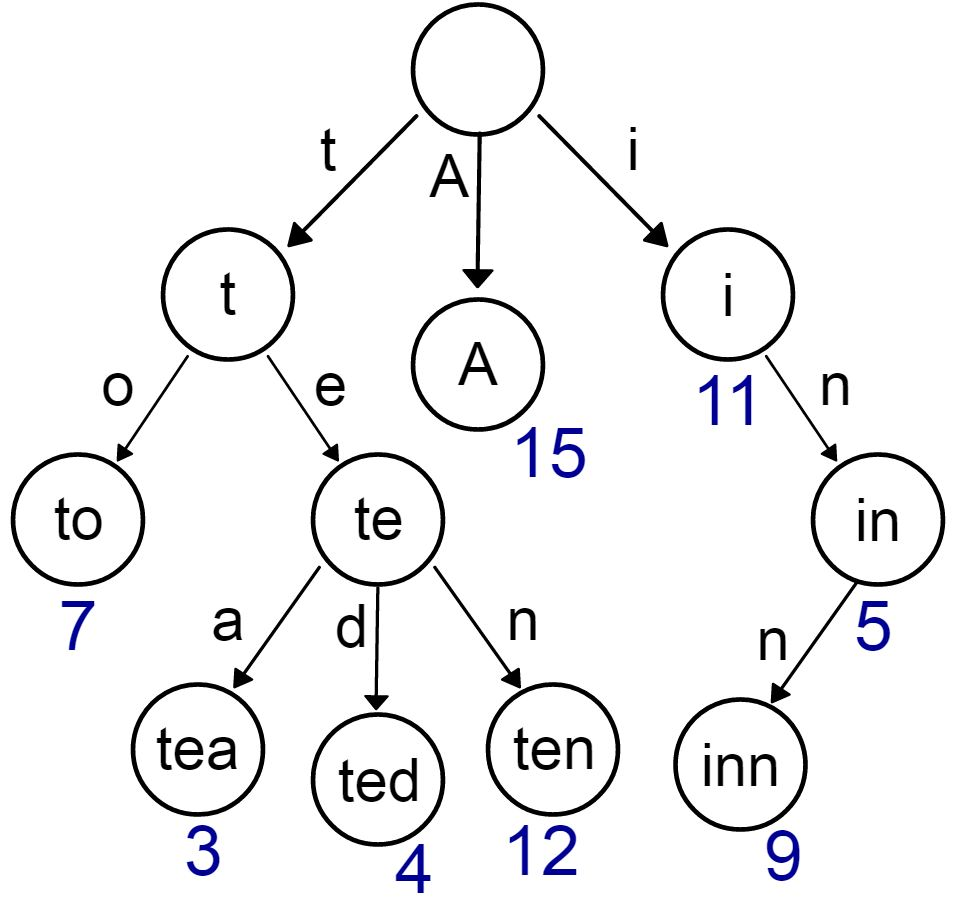
\includegraphics[width=0.5\textwidth]{svg}
		\par Trie树,又称为字典树,是一种用于存储大量字符串的树形数据结构。其每一个节点代表了一个单词或一个单词的前缀。它的优点是:利用单词的公共前缀来减少查询时间,最大限度地减少无谓的字符串比较。
		\item 使用Trie树优化动态规划算法
		\par 考虑对词典建立Trie树,并对于树上的每个点表示的字符串都求出与$S$的每一个前缀的编辑距离。节点$P$的信息可以用$P$的父节点的信息算出,这本质上与之前的DP算法相同。
		\par 我们可以对于每种编辑$L$距离求出所有有序对$(P,i)$,其中$P$表示的串与$S$的长度为$i$的前缀编辑距离为$L$。从小到大枚举$L$,当查询到的单词数量已经达到要求时,立即停止算法,就可以避免计算编辑距离过大的所有情况。
		\end{itemize}
		\par //时间复杂度:$O($词典单词总长度$\cdot$查询串的长度$)$
		\par //空间复杂度:$O($词典单词总长度$\cdot$查询串的长度$)$
		\par 优点:相较于朴素的动态规划算法,能够提高时间效率
		\par 缺点:由于需要提前建出Trie树,消耗的内存空间较大,而且时间效率仍然比较低下
	\section{局部敏感哈希算法}
	我们将问题做进一步简化,即判断两个集合的相似成度,大家普遍采用Jaccard相似度这一概念。
	\subsection{Jaccard相似度}
	对于两集合$A,B$,定义其Jaccard相似度为$$ J(A,B)=\frac{|A \cap B|}{|A \cup B|}$$
	\subsection{哈希函数}
	哈希函数是任何能将任意长度数据映射到定长数据的函数。它的值一般叫作哈希值。
	\subsection{Minhash}
	考虑所有集合的所有可能出现的元素,称其为全集$U$,我们可以从一种特殊的角度来考虑如何计算两个集合的Jaccard相似度,即遍历所有全集中的元素,不过这样代价必定是非常高的。但是我们可以采用类似的办法来估计Jaccard相似度,随机取一个$U$的排列$P$,可以将其看成一个映射$P:U\to \{1,\ldots,|U|\}$,考虑一个集合$S$中$P$值最小的元素,记为$h_S$,对于两个集合$A,B$来说,$h_A$和$h_B$相等的概率即为其Jaccard相似度,证明不是很困难,留给读者作为习题。于是我们随机选取若干个这样的$U$的排列就可以估计Jaccard相似度了,但是问题在于$|U|$的数量级一般都比较大,生成一个随机的排列很困难,所以我们可以随机选取一个$\{1,\ldots,|U|\}$到它自身的哈希函数来近似一个随机排列。
	\subsection{局部敏感哈希}
	再回到我们最初要做的事情:给一个集合,从若干个集合即词典里选出和它的Jaccard相似度最大的集合。一个朴素的想法是对当前的查询集合先做一遍Minhash,然后把它的若干个哈希值和词典中的集合的若干个哈希值逐一比对,选出其中哈希值的相同个数比较多的再两两计算Jaccard相似度,不过这样做还是比较慢的。我们可以把所有哈希函数分成若干组,把每一组中哈希值完全相同的集合划分成若干个聚类,这样对于要查询的集合我们只要遍历每一组,找到和它的这些哈希值完全相同的聚类中的元素在仔细比对即可。不过这个优化是一个很重口味,很粗糙的优化,我们做了实验,效果也很不好。不过在工业界,现实就是这样,码农们每天以卡常数为生,目前那些主流的搜索引擎中的实现不知是他们卡了多少年才卡出来的效果。但是我对这个领域的了解也不是很深入,不知道还有没有更加优秀的算法,比如说一些经过改进的自动机之类的,如果读者对这方面的研究比较有了解欢迎与我交流。
\end{document}
